\documentclass[11pt,a4paper]{report}

% ─── Packages ───
\usepackage[utf8]{inputenc}
\usepackage[T1]{fontenc}
% Font configuration
\usepackage[margin=1in, top=1.2in, bottom=1.2in]{geometry}
\usepackage{amsmath,amssymb,amsthm,mathtools}
\usepackage{xcolor}
\usepackage{titlesec}
\usepackage{titletoc}
\usepackage{fancyhdr}
\usepackage{enumitem}
\usepackage{tcolorbox}
\usepackage{booktabs}
\usepackage{graphicx}
\usepackage{hyperref}
\usepackage{cleveref}
\usepackage{tikz}
\usepackage{setspace}
\usepackage{parskip}
\usepackage{caption}
\usepackage{etoolbox}
\usepackage{array}
\usepackage{multirow}

\usetikzlibrary{arrows.meta, positioning, shapes.geometric, calc, decorations.pathmorphing, fit, backgrounds}
\tcbuselibrary{skins,breakable,theorems}

% ─── Colors ───
\definecolor{darkblue}{HTML}{1a237e}
\definecolor{accentamber}{HTML}{ff8f00}
\definecolor{deeppurple}{HTML}{311b92}
\definecolor{softgold}{HTML}{c8a951}
\definecolor{darkbg}{HTML}{121224}
\definecolor{sectionblue}{HTML}{1a3a5c}
\definecolor{subsecblue}{HTML}{2c5f8a}
\definecolor{defgreen}{HTML}{1b5e20}
\definecolor{defbg}{HTML}{e8f4e8}
\definecolor{principlecolor}{HTML}{b71c1c}
\definecolor{principlebg}{HTML}{ffebee}
\definecolor{mechblue}{HTML}{0d47a1}
\definecolor{mechbg}{HTML}{e3f2fd}
\definecolor{mathbg}{HTML}{f8f5ee}
\definecolor{notepurple}{HTML}{7b1fa2}
\definecolor{notebg}{HTML}{f3e5f5}
\definecolor{lightgray}{HTML}{f0f0f0}
\definecolor{darkgray}{HTML}{333333}
\definecolor{predcolor}{HTML}{00695c}
\definecolor{predbg}{HTML}{e0f2f1}
\definecolor{compcolor}{HTML}{4a148c}
\definecolor{compbg}{HTML}{f3e5f5}

% ─── Hyperref Setup ───
\hypersetup{
    colorlinks=true,
    linkcolor=darkblue,
    citecolor=darkblue,
    urlcolor=subsecblue,
    bookmarks=true,
    bookmarksnumbered=true,
    pdfauthor={Comprehensive Guide},
    pdftitle={Global Workspace Theory (GWT)},
    pdfsubject={Consciousness, Cognitive Architecture, Neuroscience},
}

% ─── Header/Footer ───
\pagestyle{fancy}
\fancyhf{}
\fancyhead[L]{\small\color{gray} Global Workspace Theory (GWT)}
\fancyhead[R]{\small\color{gray} Comprehensive Reading Material}
\fancyfoot[C]{\thepage}
\renewcommand{\headrulewidth}{0.4pt}
\renewcommand{\footrulewidth}{0pt}

\fancypagestyle{plain}{%
  \fancyhf{}
  \fancyfoot[C]{\thepage}
  \renewcommand{\headrulewidth}{0pt}
}

% ─── Chapter/Section Formatting ───
\titleformat{\chapter}[display]
  {\normalfont\huge\bfseries\color{darkblue}}
  {\chaptertitlename\ \thechapter}{20pt}{\Huge}
\titlespacing*{\chapter}{0pt}{-20pt}{30pt}

\titleformat{\section}
  {\normalfont\Large\bfseries\color{sectionblue}}
  {\thesection}{1em}{}
\titleformat{\subsection}
  {\normalfont\large\bfseries\color{subsecblue}}
  {\thesubsection}{1em}{}
\titleformat{\subsubsection}
  {\normalfont\normalsize\bfseries\color{darkgray}}
  {\thesubsubsection}{1em}{}

% ─── Theorem-like environments via tcolorbox ───
\newtcolorbox{principlebox}[1][]{
  enhanced, breakable,
  colback=principlebg, colframe=principlecolor,
  coltitle=white, fonttitle=\bfseries,
  title=#1,
  left=8pt, right=8pt, top=6pt, bottom=6pt,
  boxrule=0.5pt, arc=3pt,
  borderline west={3pt}{0pt}{principlecolor},
  before skip=10pt, after skip=10pt,
}

\newtcolorbox{mechbox}[1][]{
  enhanced, breakable,
  colback=mechbg, colframe=mechblue,
  coltitle=white, fonttitle=\bfseries,
  title=#1,
  left=8pt, right=8pt, top=6pt, bottom=6pt,
  boxrule=0.5pt, arc=3pt,
  borderline west={3pt}{0pt}{mechblue},
  before skip=10pt, after skip=10pt,
}

\newtcolorbox{definitionbox}[1][]{
  enhanced, breakable,
  colback=defbg, colframe=defgreen,
  coltitle=white, fonttitle=\bfseries,
  title=#1,
  left=8pt, right=8pt, top=6pt, bottom=6pt,
  boxrule=0.5pt, arc=3pt,
  borderline west={3pt}{0pt}{defgreen},
  before skip=10pt, after skip=10pt,
}

\newtcolorbox{mathbox}{
  enhanced,
  colback=mathbg, colframe=mathbg!70!black,
  left=8pt, right=8pt, top=6pt, bottom=6pt,
  boxrule=0.3pt, arc=2pt,
  before skip=8pt, after skip=8pt,
}

\newtcolorbox{notebox}[1][Note]{
  enhanced, breakable,
  colback=notebg, colframe=notepurple,
  coltitle=white, fonttitle=\bfseries,
  title=#1,
  left=8pt, right=8pt, top=6pt, bottom=6pt,
  boxrule=0.5pt, arc=3pt,
  borderline west={3pt}{0pt}{notepurple},
  before skip=10pt, after skip=10pt,
}

\newtcolorbox{predbox}[1][]{
  enhanced, breakable,
  colback=predbg, colframe=predcolor,
  coltitle=white, fonttitle=\bfseries,
  title=#1,
  left=8pt, right=8pt, top=6pt, bottom=6pt,
  boxrule=0.5pt, arc=3pt,
  borderline west={3pt}{0pt}{predcolor},
  before skip=10pt, after skip=10pt,
}

\newtcolorbox{compbox}[1][]{
  enhanced, breakable,
  colback=compbg, colframe=compcolor,
  coltitle=white, fonttitle=\bfseries,
  title=#1,
  left=8pt, right=8pt, top=6pt, bottom=6pt,
  boxrule=0.5pt, arc=3pt,
  borderline west={3pt}{0pt}{compcolor},
  before skip=10pt, after skip=10pt,
}

\newtcolorbox{examplebox}[1][Example]{
  enhanced, breakable,
  colback=lightgray, colframe=darkblue!60,
  coltitle=white, fonttitle=\bfseries,
  title=#1,
  left=8pt, right=8pt, top=6pt, bottom=6pt,
  boxrule=0.5pt, arc=3pt,
  before skip=10pt, after skip=10pt,
}

\setlength{\parindent}{0pt}
\setlength{\parskip}{6pt}

% ══════════════════════════════════════════════════════════════
\begin{document}

% ─── COVER PAGE ───
\begin{titlepage}
\begin{tikzpicture}[remember picture, overlay]
  % Background
  \fill[darkbg] (current page.south west) rectangle (current page.north east);
  % Accent line
  \fill[accentamber] ([yshift=-11cm]current page.north west) rectangle ([yshift=-10.85cm]current page.north east);
  % Decorative network nodes
  \foreach \x/\y/\r in {3/-13/0.15, 5/-12.5/0.12, 7/-13.5/0.18, 4.5/-14.5/0.1, 6.5/-14/0.14, 5/-16/0.13, 8/-15/0.11} {
    \fill[accentamber, opacity=0.2] (\x, \y) circle (\r);
  }
  \foreach \x1/\y1/\x2/\y2 in {3/-13/5/-12.5, 5/-12.5/7/-13.5, 7/-13.5/6.5/-14, 5/-12.5/4.5/-14.5, 4.5/-14.5/5/-16, 6.5/-14/8/-15, 5/-12.5/6.5/-14} {
    \draw[accentamber, opacity=0.1, line width=0.5pt] (\x1, \y1) -- (\x2, \y2);
  }
  % Large symbol
  \node[text=accentamber, opacity=0.06, scale=18] at ([yshift=-4cm, xshift=5cm]current page.center) {\textbf{GW}};
\end{tikzpicture}

\vspace*{4cm}
\begin{center}
  {\fontsize{36}{44}\selectfont\bfseries\color{white} Global Workspace\\[8pt] Theory (GWT)}\\[24pt]
  {\Large\color{gray!70} A Comprehensive Mathematical \& Conceptual Guide}\\[20pt]
  {\color{accentamber}\rule{6cm}{1pt}}\\[20pt]
  {\large\color{gray!60} From the Theater Metaphor to Computational Models\\[4pt] of Conscious Access and Broadcast}\\[40pt]
  {\color{softgold}\large Baars $\bullet$ Dehaene $\bullet$ Changeux $\bullet$ Mashour}\\[8pt]
  {\color{gray!50}\normalsize Covering Prerequisites $\bullet$ Core Principles $\bullet$ Neural Mechanisms $\bullet$ Formal Models}\\[60pt]
  {\color{gray!40}\small Comprehensive Study Material \quad$\vert$\quad February 2026}
\end{center}
\end{titlepage}

% ─── TABLE OF CONTENTS ───
\tableofcontents
\thispagestyle{plain}
\newpage


% ══════════════════════════════════════════════════════════════
\chapter{Introduction to Global Workspace Theory}
% ══════════════════════════════════════════════════════════════

\section{What is Global Workspace Theory?}

Global Workspace Theory (GWT) is one of the most influential scientific theories of consciousness, originally proposed by cognitive psychologist \textbf{Bernard Baars} in 1988. GWT provides a cognitive architecture for understanding how information becomes conscious and how conscious contents are distributed across the brain for widespread processing.

The central metaphor is that of a \textbf{theater}: consciousness is like a bright spotlight on a stage, illuminating one act at a time, while a vast audience of specialized unconscious processors sits in the darkened auditorium. Only information that enters the ``spotlight''---the \textbf{global workspace}---becomes conscious, and once there, it is \emph{broadcast} to all the audience members simultaneously.

\begin{definitionbox}[Core Claim of GWT]
Consciousness arises when information gains access to a \textbf{global workspace}---a shared, capacity-limited cognitive resource that enables the widespread \textbf{broadcasting} of information to multiple specialized, otherwise independent brain modules. Conscious access $\equiv$ global broadcast.
\end{definitionbox}

\section{Historical Context and Motivation}

GWT emerged from several converging intellectual traditions:

\textbf{(a) Cognitive science and modularity:} Jerry Fodor's (1983) influential proposal that the mind consists of specialized, informationally encapsulated \textbf{modules} (for language, face recognition, etc.) raised the question: how do these modules communicate and coordinate? GWT provides the answer: through a shared global workspace.

\textbf{(b) Artificial intelligence:} The ``blackboard architecture'' in early AI systems (Erman et al., 1980) provided a direct computational inspiration. In blackboard systems, multiple specialist modules read from and write to a shared working memory (the ``blackboard''), enabling cooperative problem-solving. GWT adapts this idea to the brain.

\textbf{(c) Attention and working memory:} Decades of research on selective attention (Broadbent, Treisman) and working memory (Baddeley) showed that consciousness is associated with a capacity-limited bottleneck. GWT identifies this bottleneck with the global workspace.

\textbf{(d) Neuroscience:} Advances in neuroimaging and electrophysiology in the 1990s--2000s revealed that conscious perception is associated with widespread, sustained brain activation, while unconscious processing remains localized---exactly as GWT predicts.

\section{The Hard Problem and GWT's Stance}

Unlike IIT, GWT does not directly attempt to solve the Hard Problem of consciousness (why there is subjective experience at all). Instead, GWT focuses on the ``\textbf{easy problems}'' (in Chalmers' terminology)---specifically, the problem of \textbf{conscious access}: what determines which information becomes conscious and which remains unconscious?

GWT is thus primarily a theory of the \textbf{function} of consciousness: what consciousness does, how it works, and what neural mechanisms underlie it. It explains the \emph{correlates} and \emph{conditions} of consciousness without claiming to explain the intrinsic nature of subjective experience.

\begin{notebox}[GWT vs.\ IIT on the Hard Problem]
IIT claims to address the Hard Problem by identifying consciousness \emph{with} integrated information. GWT is more modest: it characterizes the functional and neural architecture that determines conscious access, leaving the question of \emph{why} this architecture gives rise to experience as an open (and perhaps separate) issue. Some theorists view these as complementary rather than competing.
\end{notebox}

\section{Versions and Evolution of the Theory}

GWT has evolved significantly since Baars' original proposal:

\begin{enumerate}[leftmargin=2em]
  \item \textbf{GWT (Baars, 1988):} The original cognitive-level theory, formulated using the theater metaphor and concepts from cognitive science.
  \item \textbf{Global Neuronal Workspace Theory (GNWT)} (Dehaene, Kerszberg \& Changeux, 1998; Dehaene \& Changeux, 2011): A neurally explicit version that maps GWT onto specific brain circuits, especially prefrontal-parietal networks connected by long-range excitatory neurons.
  \item \textbf{Cognitive-Dynamic GWT (Mashour et al., 2020):} An updated framework incorporating temporal dynamics, multistability, and the role of anesthesia.
  \item \textbf{Computational models:} Formal mathematical and simulation-based implementations, including spiking neural network models by Dehaene and colleagues.
\end{enumerate}


% ══════════════════════════════════════════════════════════════
\chapter{Mathematical and Conceptual Prerequisites}
% ══════════════════════════════════════════════════════════════

This chapter reviews the mathematical and conceptual foundations needed to understand the formal models of GWT.

\section{Dynamical Systems Theory}

GWT's computational models are built on dynamical systems. A \textbf{dynamical system} describes how a state evolves over time according to a rule.

\begin{definitionbox}[Continuous Dynamical System]
A continuous dynamical system is defined by a set of ordinary differential equations (ODEs):
\[
  \frac{d\mathbf{x}}{dt} = f(\mathbf{x}, t)
\]
where $\mathbf{x}(t) \in \mathbb{R}^n$ is the state vector (e.g., firing rates of neural populations) and $f$ specifies the dynamics. In neural models, $f$ encodes the connectivity, excitation/inhibition balance, and nonlinear activation of neural populations.
\end{definitionbox}

Key concepts relevant to GWT:
\begin{itemize}[leftmargin=1.5em]
  \item \textbf{Attractors:} Stable states toward which the system evolves. In GWT, a conscious percept may correspond to the system settling into a global attractor.
  \item \textbf{Bifurcations:} Qualitative changes in system behavior as parameters change. The transition from unconscious to conscious processing may involve a bifurcation (sudden ignition).
  \item \textbf{Bistability / Multistability:} The coexistence of multiple stable states. The global workspace may switch between competing representations.
\end{itemize}

\section{Neural Population Models}

The neural implementations of GWT use population-level models, where the fundamental variable is the average firing rate or membrane potential of a neural \emph{population} (a group of similar neurons).

\subsection{Wilson--Cowan Model}

The Wilson--Cowan equations describe the interaction between excitatory ($E$) and inhibitory ($I$) neural populations:

\begin{mathbox}
\vspace{-6pt}
\begin{align}
  \tau_E \frac{dE}{dt} &= -E + S_E\!\left(w_{EE} E - w_{EI} I + I_{\text{ext}}^E\right) \label{eq:wc_e}\\[6pt]
  \tau_I \frac{dI}{dt} &= -I + S_I\!\left(w_{IE} E - w_{II} I + I_{\text{ext}}^I\right) \label{eq:wc_i}
\end{align}
\vspace{-8pt}
\end{mathbox}

where $\tau_E, \tau_I$ are time constants, $w_{XY}$ are connection weights, $I_{\text{ext}}$ is external input, and $S(\cdot)$ is a sigmoidal activation function:
\[
  S(x) = \frac{1}{1 + e^{-\beta(x - \theta)}} - \frac{1}{1 + e^{\beta\theta}}
\]
with gain $\beta$ and threshold $\theta$. These equations form the building blocks for multi-area models of the global workspace.

\subsection{Mean-Field Approximations}

For large networks, \textbf{mean-field theory} replaces the detailed behavior of individual neurons with population-averaged quantities. For a population of $N$ neurons with mean firing rate $\nu$:

\begin{mathbox}
\vspace{-8pt}
\[
  \nu = \Phi\!\left(\mu_V,\; \sigma_V^2\right)
\]
\vspace{-10pt}
\end{mathbox}

where $\mu_V$ and $\sigma_V^2$ are the mean and variance of the membrane potential, and $\Phi$ is a transfer function derived from single-neuron properties (e.g., the frequency-current or f-I curve). The inputs to each population include:
\[
  \mu_V = \sum_j w_j \nu_j + I_{\text{ext}}, \qquad \sigma_V^2 = \sum_j w_j^2 \nu_j \tau_{\text{syn}}
\]
where the sum is over all presynaptic populations $j$.

\section{Information Theory for Neural Coding}

Information theory provides tools for quantifying how much information neural activity carries about stimuli.

\subsection{Mutual Information in Neural Coding}

The mutual information between a stimulus $S$ and a neural response $R$:
\[
  I(S; R) = H(R) - H(R \mid S) = \sum_{s, r} p(s, r) \log_2 \frac{p(s, r)}{p(s)\, p(r)}
\]

In the context of GWT, this quantifies how much information about a stimulus is carried by neural activity in a given brain area. Conscious access (broadcast) should increase $I(S; R)$ for \emph{distant} brain areas.

\subsection{Transfer Entropy}

\textbf{Transfer entropy} quantifies directed information flow between time series---essential for measuring broadcast dynamics:

\begin{mathbox}
\vspace{-8pt}
\[
  T_{X \to Y} = \sum p\!\left(y_{t+1}, y_t^{(k)}, x_t^{(l)}\right) \log_2 \frac{p\!\left(y_{t+1} \mid y_t^{(k)}, x_t^{(l)}\right)}{p\!\left(y_{t+1} \mid y_t^{(k)}\right)}
\]
\vspace{-10pt}
\end{mathbox}

where $y_t^{(k)}$ and $x_t^{(l)}$ denote the past $k$ and $l$ values of $Y$ and $X$ respectively. High transfer entropy from workspace regions to sensory areas indicates global broadcast.

\subsection{Granger Causality}

A linear counterpart to transfer entropy, \textbf{Granger causality} tests whether past values of $X$ improve the prediction of $Y$ beyond $Y$'s own past:
\[
  Y_t = \sum_{i=1}^{p} a_i Y_{t-i} + \sum_{j=1}^{q} b_j X_{t-j} + \varepsilon_t
\]
$X$ Granger-causes $Y$ if the coefficients $b_j$ are jointly significant ($F$-test). This is widely used in neuroimaging to measure effective connectivity and information flow during conscious vs.\ unconscious processing.

\section{Signal Detection Theory}

GWT's empirical predictions are often tested using paradigms from \textbf{signal detection theory} (SDT), which provides a mathematical framework for analyzing perceptual decisions.

\begin{definitionbox}[Signal Detection: $d'$ and Criterion $c$]
Given a signal+noise distribution $\mathcal{N}(\mu_S, \sigma^2)$ and a noise-only distribution $\mathcal{N}(\mu_N, \sigma^2)$:
\[
  d' = \frac{\mu_S - \mu_N}{\sigma}
\]
measures discriminability (sensitivity), independent of response bias. The criterion:
\[
  c = -\frac{1}{2}\left[z(\text{hit rate}) + z(\text{false alarm rate})\right]
\]
measures the observer's decision threshold. In GWT, conscious access corresponds to stimuli exceeding a \emph{threshold} for global ignition, and SDT provides tools for separating sensitivity from criterion effects.
\end{definitionbox}

\section{Graph Theory for Brain Networks}

The global workspace is realized by a network of brain regions. Graph-theoretic measures characterize its structure.

\begin{definitionbox}[Key Network Measures]
For a graph $G = (V, E)$ with adjacency matrix $A$:
\begin{itemize}[leftmargin=1.5em]
  \item \textbf{Degree:} $k_i = \sum_j A_{ij}$ --- number of connections of node $i$.
  \item \textbf{Clustering coefficient:} $C_i = \frac{2 |\{e_{jk} : v_j, v_k \in N_i, e_{jk} \in E\}|}{k_i(k_i - 1)}$ --- local connectivity.
  \item \textbf{Path length:} $L = \frac{1}{n(n{-}1)} \sum_{i \neq j} d(i,j)$ --- average shortest path.
  \item \textbf{Small-world index:} $\sigma = \frac{C/C_{\text{random}}}{L/L_{\text{random}}}$ --- high clustering with short paths.
  \item \textbf{Hub nodes:} Nodes with disproportionately high degree or betweenness centrality.
\end{itemize}
The global workspace is hypothesized to rely on \textbf{hub nodes} with high betweenness centrality that enable efficient broadcast.
\end{definitionbox}


% ══════════════════════════════════════════════════════════════
\chapter{Core Principles of GWT}
% ══════════════════════════════════════════════════════════════

This chapter details the foundational principles of GWT. Unlike IIT's axiom-based structure, GWT is organized around a set of functional principles derived from cognitive science and neuroscience.

\section{Principle 1: Modularity and Specialization}

\begin{principlebox}[Principle 1 --- Modularity]
The brain consists of a large number of specialized, semi-autonomous \textbf{processors} (modules), each handling a specific type of information (e.g., color, motion, faces, language syntax). These modules operate largely in \textbf{parallel} and \textbf{unconsciously}.
\end{principlebox}

Examples of specialized modules include the fusiform face area (FFA) for face processing, area V4 for color, area MT/V5 for motion, Wernicke's area for language comprehension, and the amygdala for threat detection. Each module can process information rapidly and automatically without requiring conscious awareness.

The key insight: most of what the brain does is \emph{unconscious}. The vast majority of neural processing occurs in specialized modules that never enter awareness. Consciousness is the exception, not the rule.

\section{Principle 2: The Global Workspace as Integrative Hub}

\begin{principlebox}[Principle 2 --- The Global Workspace]
There exists a \textbf{global workspace}---a capacity-limited, shared cognitive resource---that allows information from any one module to be made available to \textbf{all other modules simultaneously}. This workspace acts as a central integration and broadcasting hub.
\end{principlebox}

The global workspace is not a single brain region but a \textbf{distributed network} of neurons, primarily involving long-range cortical connections. In the neural implementation (GNWT), it is associated with:
\begin{itemize}[leftmargin=1.5em]
  \item Prefrontal cortex (especially dorsolateral PFC)
  \item Parietal cortex (especially posterior parietal regions)
  \item Anterior cingulate cortex (ACC)
  \item Long-range cortico-cortical axons connecting these areas
\end{itemize}

The workspace is \textbf{capacity-limited}: only one coherent representation (or a very small number) can occupy the workspace at a time. This explains the well-known bottleneck of consciousness---we can only be conscious of one thing (or a very few things) at a time.

\section{Principle 3: Competition and Selection}

\begin{principlebox}[Principle 3 --- Competition for Access]
Multiple unconscious processors compete for access to the global workspace. This competition is governed by \textbf{bottom-up salience} (stimulus strength, novelty, emotional valence) and \textbf{top-down attention} (goals, expectations, task relevance). Only the ``winning'' representation gains access.
\end{principlebox}

The competition can be modeled as a winner-take-all (WTA) dynamics:

\begin{mathbox}
\vspace{-6pt}
\[
  \tau \frac{dx_i}{dt} = -x_i + f\!\left(\sum_j w_{ij}^{\text{local}} x_j + I_i^{\text{ext}} - \alpha \sum_{k \neq i} x_k\right)
\]
\vspace{-8pt}
\end{mathbox}

where $x_i$ is the activity of the $i$-th competing representation, $w^{\text{local}}$ are local recurrent connections (self-amplification), $I^{\text{ext}}$ is external drive, $\alpha$ controls lateral inhibition (competition), and $f$ is a nonlinear activation function. The representation with the strongest combined bottom-up and top-down support wins the competition and enters the workspace.

\section{Principle 4: Ignition and Broadcast}

\begin{principlebox}[Principle 4 --- Ignition]
When a representation wins the competition and enters the global workspace, it triggers a sudden, self-reinforcing, nonlinear \textbf{ignition}---a rapid amplification of activity through recurrent loops between workspace neurons. This ignition constitutes the \textbf{neural correlate of conscious access}.
\end{principlebox}

Ignition is the signature event in GNWT. It is characterized by:
\begin{itemize}[leftmargin=1.5em]
  \item A sudden, \textbf{nonlinear} transition from localized to widespread activity
  \item Self-sustaining activity through positive feedback loops
  \item \textbf{All-or-none} character: ignition either occurs fully or not at all
  \item A time delay ($\sim$200--300 ms after stimulus onset)
  \item Associated electrophysiological signatures (P3b wave, late sustained activity, gamma synchrony)
\end{itemize}

\begin{principlebox}[Principle 5 --- Global Broadcast]
Following ignition, the contents of the global workspace are \textbf{broadcast} to all connected modules simultaneously. This broadcast makes the information available for diverse cognitive operations: verbal report, memory encoding, planning, emotional evaluation, and voluntary action.
\end{principlebox}

The broadcast is the functional essence of consciousness in GWT: it is the mechanism by which a piece of information transitions from being processed locally and unconsciously to being \emph{globally available} and conscious.

\section{Principle 6: Conscious vs.\ Unconscious Processing}

\begin{principlebox}[Principle 6 --- The Conscious/Unconscious Divide]
\textbf{Unconscious} processing is: parallel, fast, automatic, capacity-unlimited, localized, and modular. \textbf{Conscious} processing is: serial (one content at a time), relatively slow, effortful, capacity-limited, distributed, and integrated.
\end{principlebox}

This leads to a clear taxonomy:

\begin{center}
\renewcommand{\arraystretch}{1.3}
\begin{tabular}{>{\raggedright}p{4cm} >{\raggedright}p{4.5cm} >{\raggedright\arraybackslash}p{4.5cm}}
  \toprule
  \textbf{Property} & \textbf{Unconscious Processing} & \textbf{Conscious Processing} \\
  \midrule
  Capacity & Unlimited (many modules) & Severely limited \\
  Speed & Fast ($<$200 ms) & Slow ($>$300 ms) \\
  Processing mode & Parallel & Serial \\
  Neural scope & Local, modular & Global, distributed \\
  Flexibility & Fixed, automatic & Flexible, voluntary \\
  Reportability & Not reportable & Reportable \\
  Information sharing & Limited to local circuits & Broadcast to all modules \\
  \bottomrule
\end{tabular}
\end{center}


% ══════════════════════════════════════════════════════════════
\chapter{The Global Neuronal Workspace (GNWT)}
% ══════════════════════════════════════════════════════════════

This chapter covers the neurally explicit version of GWT, developed primarily by Stanislas Dehaene and Jean-Pierre Changeux.

\section{Architecture of the Global Neuronal Workspace}

\subsection{Workspace Neurons}

The global neuronal workspace consists of a specific population of neurons characterized by:

\begin{mechbox}[Workspace Neuron Properties]
\begin{enumerate}[leftmargin=1.5em]
  \item \textbf{Long-range axons:} Workspace neurons have long-range cortico-cortical axons that project across distant brain areas. They are concentrated in layers II/III of the cortex.
  \item \textbf{Prefrontal-parietal distribution:} They are especially dense in prefrontal and parietal cortex but are found throughout the cortex.
  \item \textbf{Recurrent connectivity:} Workspace neurons form dense recurrent loops with each other, enabling self-sustaining activity.
  \item \textbf{Top-down projections:} They project back to sensory areas, modulating local processing through feedback connections.
\end{enumerate}
\end{mechbox}

\subsection{Peripheral Processors}

Contrasted with workspace neurons are the \textbf{peripheral processors}---specialized cortical and subcortical areas that perform specific computations (visual processing, auditory analysis, motor planning, etc.). These processors:
\begin{itemize}[leftmargin=1.5em]
  \item Have primarily local, short-range connections
  \item Operate automatically and in parallel
  \item Can process information without workspace involvement (unconscious processing)
  \item Compete for access to the workspace via bottom-up signals
\end{itemize}

\subsection{Connectivity Architecture}

The GNWT architecture can be summarized as a \textbf{hub-and-spoke} model:

\begin{center}
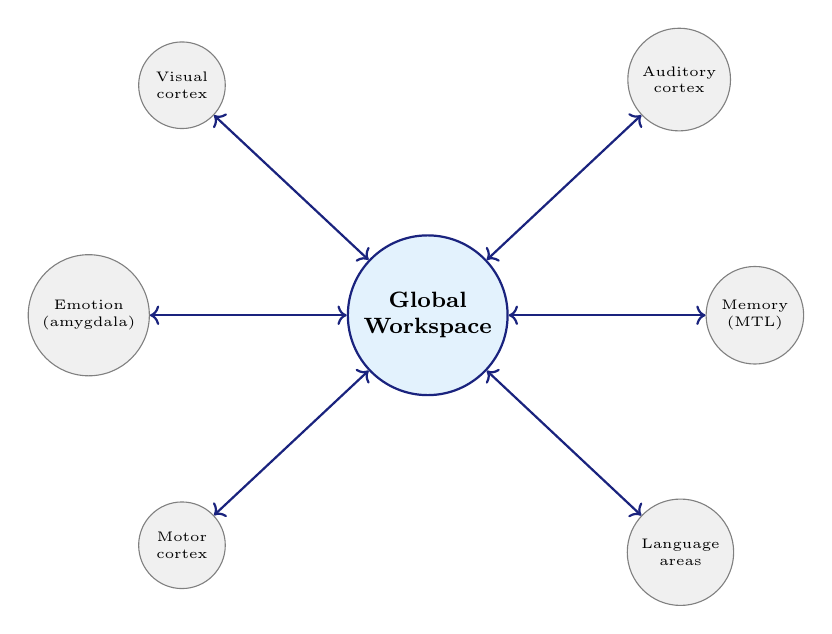
\begin{tikzpicture}[
    node distance=2.5cm,
    hub/.style={circle, draw=darkblue, fill=mechbg, thick, minimum size=1.5cm, font=\footnotesize\bfseries, align=center},
    spoke/.style={circle, draw=gray, fill=lightgray, minimum size=1.1cm, font=\tiny, align=center},
    hubline/.style={-{Stealth[length=3mm]}, thick, darkblue},
    spokeline/.style={-{Stealth[length=2mm]}, gray},
  ]
  % Hub
  \node[hub] (gw) {Global\\Workspace};
  % Spokes
  \node[spoke, above left=1.8cm and 2cm of gw] (v) {Visual\\cortex};
  \node[spoke, above right=1.8cm and 2cm of gw] (a) {Auditory\\cortex};
  \node[spoke, below left=1.8cm and 2cm of gw] (m) {Motor\\cortex};
  \node[spoke, below right=1.8cm and 2cm of gw] (l) {Language\\areas};
  \node[spoke, left=2.5cm of gw] (e) {Emotion\\(amygdala)};
  \node[spoke, right=2.5cm of gw] (mem) {Memory\\(MTL)};
  % Bidirectional connections
  \draw[hubline, <->] (gw) -- (v);
  \draw[hubline, <->] (gw) -- (a);
  \draw[hubline, <->] (gw) -- (m);
  \draw[hubline, <->] (gw) -- (l);
  \draw[hubline, <->] (gw) -- (e);
  \draw[hubline, <->] (gw) -- (mem);
\end{tikzpicture}
\end{center}
\vspace{-4pt}
{\small\centering\textit{Figure: Hub-and-spoke architecture. The global workspace receives input from and broadcasts to all specialized processors.}\par}

\section{The Ignition Dynamics: Mathematical Model}

Dehaene and Changeux (2005) formalized ignition using a neural network model. The key is the interaction between local sensory processors and the global workspace, mediated by long-range excitatory connections.

\subsection{Two-Population Model}

Consider two coupled populations: a sensory population ($S$) and a workspace population ($W$). Their mean firing rates evolve according to:

\begin{mathbox}
\vspace{-6pt}
\begin{align}
  \tau_S \frac{d\nu_S}{dt} &= -\nu_S + \Phi_S\!\left(w_{SS}\,\nu_S + w_{SW}\,\nu_W + I_{\text{stim}}\right) \label{eq:sensory}\\[6pt]
  \tau_W \frac{d\nu_W}{dt} &= -\nu_W + \Phi_W\!\left(w_{WW}\,\nu_W + w_{WS}\,\nu_S + I_{\text{top-down}}\right) \label{eq:workspace}
\end{align}
\vspace{-8pt}
\end{mathbox}

where:
\begin{itemize}[leftmargin=1.5em]
  \item $\nu_S, \nu_W$: mean firing rates of sensory and workspace populations
  \item $\tau_S, \tau_W$: time constants (workspace often slower, $\tau_W > \tau_S$)
  \item $w_{SS}$: local recurrence in sensory area
  \item $w_{WW}$: recurrence within workspace (critical for ignition)
  \item $w_{SW}, w_{WS}$: long-range connections (bottom-up and top-down)
  \item $\Phi(\cdot)$: sigmoidal transfer function
  \item $I_{\text{stim}}$: sensory input; $I_{\text{top-down}}$: attentional modulation
\end{itemize}

\subsection{Ignition as a Bifurcation}

The key mathematical insight is that ignition corresponds to a \textbf{saddle-node bifurcation}. As $I_{\text{stim}}$ increases:

\begin{enumerate}[leftmargin=2em]
  \item For weak stimuli ($I_{\text{stim}} < I_{\text{crit}}$): the system has only one stable fixed point with $\nu_W \approx 0$ (no workspace activity). The stimulus is processed locally but \textbf{not} consciously perceived.
  \item At the critical threshold ($I_{\text{stim}} = I_{\text{crit}}$): a saddle-node bifurcation occurs, creating a new stable fixed point with $\nu_W \gg 0$ (high workspace activity).
  \item For strong stimuli ($I_{\text{stim}} > I_{\text{crit}}$): the system rapidly transitions to the high-activity state---\textbf{ignition}. The stimulus enters the workspace and is consciously perceived.
\end{enumerate}

\begin{mathbox}
\vspace{-6pt}
The critical threshold can be estimated from the fixed-point equation. At the bifurcation:
\[
  \frac{\partial}{\partial \nu_W} \left[-\nu_W + \Phi_W(w_{WW}\,\nu_W + \ldots)\right] = 0
\]
which gives $w_{WW} \cdot \Phi_W'(\cdot) = 1$. This shows that ignition requires sufficiently strong recurrent workspace connectivity ($w_{WW}$) and/or sufficiently strong bottom-up input.
\vspace{-4pt}
\end{mathbox}

The all-or-none character of conscious perception emerges naturally: below threshold, $\nu_W \approx 0$ (unconscious); above threshold, $\nu_W$ jumps to a high value (conscious). There is no ``partial'' ignition---this is a nonlinear phase transition.

\subsection{Top-Down Modulation and Attention}

Top-down attention modulates the ignition threshold. In the model, $I_{\text{top-down}}$ effectively lowers $I_{\text{crit}}$, making it easier for stimuli to reach consciousness:

\[
  I_{\text{crit}}^{\text{attended}} < I_{\text{crit}}^{\text{unattended}}
\]

This explains why attended stimuli are more easily perceived: attention pre-activates workspace neurons, bringing them closer to the ignition threshold.

\section{Multi-Area Spiking Model}

Dehaene, Changeux, and colleagues (2003) developed a more detailed model using spiking neurons organized into multiple cortical columns. Each column contains:

\begin{itemize}[leftmargin=1.5em]
  \item 80\% excitatory pyramidal neurons (further divided into layers)
  \item 20\% inhibitory interneurons
  \item AMPA and NMDA excitatory synapses
  \item GABA$_A$ inhibitory synapses
\end{itemize}

Columns are connected locally (within a cortical area) and long-range (via workspace neurons). The model implements:

\[
  C_m \frac{dV_i}{dt} = -g_L(V_i - V_L) - \sum_{\text{syn}} I_{\text{syn},i} + I_{\text{ext},i}
\]

where $V_i$ is the membrane potential of neuron $i$, $g_L$ is the leak conductance, and $I_{\text{syn}}$ includes AMPA, NMDA, and GABA$_A$ synaptic currents. Key findings from these simulations:

\begin{predbox}[Simulation Results]
\begin{enumerate}[leftmargin=1.5em]
  \item \textbf{Subliminal processing:} Weak stimuli activate sensory columns transiently but fail to ignite workspace neurons. Activity dies out quickly.
  \item \textbf{Ignition:} Sufficiently strong stimuli trigger a sudden, self-sustaining activation of workspace neurons across multiple areas, lasting several hundred milliseconds.
  \item \textbf{Masking:} A second stimulus presented shortly after the first can prevent ignition by disrupting the bottom-up signal before it reaches the workspace---reproducing masking effects in psychophysics.
  \item \textbf{Attentional blink:} While the workspace processes one stimulus, it is temporarily unavailable for a second stimulus, reproducing the attentional blink phenomenon.
\end{enumerate}
\end{predbox}


% ══════════════════════════════════════════════════════════════
\chapter{Formal Computational Models}
% ══════════════════════════════════════════════════════════════

\section{The Broadcast Formalism}

Let us formalize the broadcast operation. Consider a set of $N$ modules $\{M_1, M_2, \ldots, M_N\}$, each with an internal state $\mathbf{x}_i(t) \in \mathbb{R}^{d_i}$. The workspace state is $\mathbf{w}(t) \in \mathbb{R}^{d_w}$.

\begin{definitionbox}[Broadcast Dynamics]
The dynamics of the system are:
\begin{align}
  \tau_i \frac{d\mathbf{x}_i}{dt} &= F_i(\mathbf{x}_i) + G_i(\mathbf{w}) + \mathbf{u}_i(t) \label{eq:module_dyn}\\[6pt]
  \tau_w \frac{d\mathbf{w}}{dt} &= F_w(\mathbf{w}) + \sum_{i=1}^{N} \alpha_i(t)\, H_i(\mathbf{x}_i) \label{eq:workspace_dyn}
\end{align}

where:
\begin{itemize}[leftmargin=1.5em]
  \item $F_i$: internal dynamics of module $i$; \; $F_w$: internal workspace dynamics
  \item $G_i(\mathbf{w})$: broadcast signal from workspace to module $i$ (top-down)
  \item $H_i(\mathbf{x}_i)$: input from module $i$ to workspace (bottom-up)
  \item $\alpha_i(t) \in [0, 1]$: gating variable (attention/competition result)
  \item $\mathbf{u}_i(t)$: external input to module $i$
\end{itemize}
\end{definitionbox}

The \textbf{broadcast} is realized by the $G_i(\mathbf{w})$ term: once the workspace is activated (ignited), its state $\mathbf{w}$ is transmitted to \emph{all} modules $M_i$, modulating their processing.

\subsection{Competition via Gating}

The gating variables $\alpha_i(t)$ implement competition. In the simplest case:
\[
  \alpha_i = \frac{e^{\beta s_i}}{\sum_j e^{\beta s_j}}
\]
where $s_i = \|\mathbf{x}_i\| + b_i$ combines bottom-up signal strength $\|\mathbf{x}_i\|$ with top-down bias $b_i$, and $\beta$ is an inverse temperature parameter. As $\beta \to \infty$, this becomes a hard winner-take-all: only the module with the highest $s_i$ gains access ($\alpha_i \to 1$, all others $\to 0$).

\section{Information-Theoretic Characterization}

GWT's broadcast can be characterized information-theoretically.

\subsection{Broadcast as Information Gain}

Define the \textbf{information gain} from broadcast for module $i$ as:
\begin{mathbox}
\vspace{-8pt}
\[
  \Delta I_i = I(\mathbf{x}_i;\; S) \big|_{\text{after broadcast}} - I(\mathbf{x}_i;\; S) \big|_{\text{before broadcast}}
\]
\vspace{-10pt}
\end{mathbox}

where $S$ is the stimulus that entered the workspace. Before broadcast, module $i$ has no information about $S$ (if it was processed by a different module). After broadcast, it receives information via the workspace. The total information gain across all modules:
\[
  \Delta I_{\text{total}} = \sum_{i=1}^{N} \Delta I_i
\]

This quantifies the ``amplification'' effect of consciousness: a single piece of information, once broadcast, becomes available across the entire brain.

\subsection{Workspace Capacity and Information Bottleneck}

The capacity limitation of the workspace can be formalized using the \textbf{information bottleneck} framework (Tishby et al., 1999). The workspace $W$ compresses input information $X$ while preserving information about the relevant variable $Y$:

\begin{mathbox}
\vspace{-8pt}
\[
  \min_{p(w|x)} \Big[\, I(X; W) - \beta\, I(W; Y)\,\Big]
\]
\vspace{-10pt}
\end{mathbox}

where $I(X; W)$ is the compression cost (limited by workspace capacity) and $I(W; Y)$ is the preserved relevant information. The parameter $\beta$ trades off compression against information preservation. This formalization explains why consciousness is both limited (compressed) and informative (preserving relevant information).

\section{Bayesian Formulation}

GWT has also been connected to Bayesian inference. The workspace maintains a probability distribution over hypotheses, updated by Bayes' rule when new information enters:

\[
  p(H \mid D) = \frac{p(D \mid H)\, p(H)}{p(D)}
\]

Conscious perception corresponds to the posterior $p(H \mid D)$ after sufficient evidence accumulation. The ignition threshold corresponds to a decision boundary in the Bayesian framework---the point at which the posterior probability of one hypothesis exceeds a criterion:

\[
  \text{Conscious access:} \quad p(H_1 \mid D) > \theta_{\text{crit}}
\]

This connects GWT to accumulator models (drift-diffusion models) used in decision neuroscience. The decision variable $x(t)$ accumulates evidence:
\[
  dx = \mu\, dt + \sigma\, dW_t
\]
where $\mu$ is the drift rate (signal strength) and $\sigma\, dW_t$ is noise. Conscious perception occurs when $x(t)$ first crosses the boundary $\theta$. The mean reaction time is $\bar{T} = \theta / \mu$.


% ══════════════════════════════════════════════════════════════
\chapter{Neural Signatures of Conscious Access}
% ══════════════════════════════════════════════════════════════

GNWT makes specific predictions about the neural signatures that distinguish conscious from unconscious processing. These have been extensively tested.

\section{The P3b / P300 Wave}

The most robust electrophysiological marker of conscious access is the \textbf{P3b component}---a positive-going ERP wave peaking $\sim$300--500 ms after stimulus onset at parietal electrodes.

\begin{mechbox}[P3b as Ignition Marker]
According to GNWT:
\begin{itemize}[leftmargin=1.5em]
  \item The P3b reflects the \textbf{ignition} of the global workspace.
  \item It is present for consciously perceived stimuli and \textbf{absent} for unperceived stimuli.
  \item Its latency ($\sim$300 ms) reflects the time needed for bottom-up signals to reach and activate the workspace.
  \item Its widespread scalp topography reflects the global distribution of workspace neurons.
  \item Its amplitude correlates with subjective confidence in perception.
\end{itemize}
\end{mechbox}

\section{Late Sustained Activity}

Beyond the P3b, conscious perception is associated with \textbf{late sustained activity} ($>$300 ms) in prefrontal and parietal areas, as measured by fMRI, MEG, and intracranial recordings. This sustained activity reflects the self-maintaining dynamics of the ignited workspace and the ongoing broadcast.

\section{Gamma-Band Synchrony and Long-Range Connectivity}

Conscious access is associated with increased \textbf{gamma-band} ($30$--$100$ Hz) oscillatory synchrony between distant brain areas:

\begin{mathbox}
\vspace{-6pt}
\textbf{Phase-locking value (PLV)} between signals $x(t)$ and $y(t)$:
\[
  \text{PLV} = \left| \frac{1}{T} \sum_{t=1}^{T} e^{i\,[\phi_x(t) - \phi_y(t)]} \right|
\]
where $\phi_x(t)$ and $\phi_y(t)$ are the instantaneous phases extracted via the Hilbert transform or wavelet analysis. PLV $\approx 1$ indicates perfect phase synchrony; PLV $\approx 0$ indicates no consistent phase relationship.
\vspace{-4pt}
\end{mathbox}

GNWT predicts that conscious perception should show increased long-range PLV (especially in beta/gamma bands), reflecting the coordinated activity of the ignited workspace. This has been confirmed experimentally.

\section{The ``All-or-None'' Pattern}

A distinctive prediction of GNWT is that the transition from unconscious to conscious processing is \textbf{nonlinear} (all-or-none), not gradual. This has been tested using:

\begin{enumerate}[leftmargin=2em]
  \item \textbf{Masking paradigms:} Varying stimulus-mask SOA reveals a sharp threshold---below a critical SOA, perception is at chance; above it, perception is nearly perfect. Intermediate performance reflects trial-by-trial variability (ignition or no ignition), not graded awareness.
  \item \textbf{fMRI studies:} Activity in prefrontal/parietal areas shows a bimodal distribution (high or low), not a continuum, correlated with reports of seeing vs.\ not seeing.
  \item \textbf{Single-trial analysis:} Trial-by-trial neural signatures cluster into two distinct states (ignited/not ignited), with the probability of ignition varying smoothly with stimulus strength.
\end{enumerate}


% ══════════════════════════════════════════════════════════════
\chapter{Key Experimental Paradigms}
% ══════════════════════════════════════════════════════════════

\section{Visual Masking}

In \textbf{backward masking}, a brief target stimulus is followed by a mask after a variable stimulus-onset asynchrony (SOA). GWT predicts:

\begin{itemize}[leftmargin=1.5em]
  \item At short SOAs ($<$50 ms): the mask disrupts bottom-up signals before ignition---target is invisible.
  \item At long SOAs ($>$100 ms): ignition has time to occur---target is seen.
  \item At intermediate SOAs: trial-by-trial variability (all-or-none ignition on each trial).
\end{itemize}

Dehaene et al.\ (2001) showed exactly this pattern using fMRI and ERPs, demonstrating bimodal brain responses consistent with ignition dynamics.

\section{The Attentional Blink}

When two targets (T1 and T2) are embedded in a rapid stream, T2 is often missed if it appears 200--500 ms after T1. GWT explains this as a \textbf{workspace refractory period}: while the workspace processes T1 (ignition + broadcast), it is temporarily unavailable for T2.

The mathematical model predicts the characteristic U-shaped function of T2 detection vs.\ T1--T2 lag:
\begin{itemize}[leftmargin=1.5em]
  \item Lag 1 (very short): T2 can ``sneak in'' during T1 ignition (Lag-1 sparing)
  \item Lag 2--5 ($\sim$200--500 ms): workspace occupied by T1, T2 is missed (blink)
  \item Lag 6+ ($>$500 ms): T1 processing complete, workspace available again
\end{itemize}

\section{Binocular Rivalry}

When different images are presented to each eye, perception alternates between them. GWT explains this as \textbf{alternating ignition}: each image competes for workspace access, and the currently conscious image maintains ignition until it is displaced by the competing image.

The alternation dynamics can be modeled with coupled oscillators:
\begin{align}
  \tau \frac{dx_1}{dt} &= -x_1 + f(I_1 - \beta\, x_2 - a(t)\, x_1) \\
  \tau \frac{dx_2}{dt} &= -x_2 + f(I_2 - \beta\, x_1 - a(t)\, x_2)
\end{align}
where $x_1, x_2$ are activities of the two percepts, $\beta$ is mutual inhibition, and $a(t)$ is an adaptation term that weakens the currently dominant percept over time, allowing the other to win.

The mean dominance duration $\bar{T}$ follows a gamma distribution, consistent with a noise-driven switching process:
\[
  p(T) = \frac{T^{k-1} e^{-T/\theta}}{\theta^k \,\Gamma(k)}
\]
where $k$ and $\theta$ are the shape and scale parameters.

\section{Inattentional Blindness and Change Blindness}

These phenomena demonstrate that even physically salient stimuli can fail to reach consciousness if attention is directed elsewhere---directly supporting the role of top-down attention in gating workspace access.


% ══════════════════════════════════════════════════════════════
\chapter{Consciousness Under Altered States}
% ══════════════════════════════════════════════════════════════

\section{General Anesthesia}

GWT provides a natural explanation for the loss of consciousness under anesthesia. Anesthetic agents (e.g., propofol, sevoflurane) disrupt consciousness by:

\begin{enumerate}[leftmargin=2em]
  \item \textbf{Disrupting long-range connectivity:} Anesthetics preferentially disrupt the long-range cortico-cortical connections that constitute the workspace, while leaving local processing relatively intact.
  \item \textbf{Preventing ignition:} By reducing recurrent excitation ($w_{WW}$) and increasing inhibition, anesthetics raise the ignition threshold $I_{\text{crit}}$ above any achievable sensory input.
  \item \textbf{Breaking the broadcast:} Even if local sensory processing persists, the workspace cannot amplify and distribute the information.
\end{enumerate}

Empirically, this is supported by studies showing that propofol specifically disrupts frontoparietal connectivity and prefrontal cortex feedback activity, while sensory-evoked responses in primary sensory cortex remain largely intact.

\section{Sleep and Dreaming}

\textbf{NREM sleep:} During deep sleep, cortical connectivity breaks down---neurons enter bistable ``up'' and ``down'' states, preventing sustained workspace ignition. GWT predicts reduced consciousness during NREM, consistent with the phenomenology.

\textbf{REM sleep / Dreaming:} During REM sleep, cortical connectivity is partially restored, and workspace ignition can occur---but driven by internal signals rather than external stimuli. This produces the vivid but often bizarre conscious experiences of dreaming.

\section{Disorders of Consciousness}

The GWT framework helps classify disorders of consciousness:
\begin{itemize}[leftmargin=1.5em]
  \item \textbf{Vegetative state:} Intact local processing but no global ignition (workspace structurally or functionally disconnected).
  \item \textbf{Minimally conscious state:} Intermittent workspace ignition (partial recovery of long-range connectivity).
  \item \textbf{Locked-in syndrome:} Intact workspace and consciousness but disrupted motor output---the workspace is ignited, but the broadcast to motor systems is blocked.
\end{itemize}


% ══════════════════════════════════════════════════════════════
\chapter{GWT vs.\ Other Theories}
% ══════════════════════════════════════════════════════════════

\section{GWT vs.\ Integrated Information Theory (IIT)}

\begin{compbox}[Key Differences: GWT vs.\ IIT]
\renewcommand{\arraystretch}{1.4}
\begin{tabular}{>{\raggedright}p{3cm} >{\raggedright}p{5cm} >{\raggedright\arraybackslash}p{5cm}}
  \toprule
  \textbf{Dimension} & \textbf{GWT / GNWT} & \textbf{IIT} \\
  \midrule
  What is consciousness? & Global broadcast/access & Integrated information ($\Phi$) \\
  Starting point & Function/mechanism & Phenomenology (axioms) \\
  Hard Problem & Not directly addressed & Claimed to be addressed \\
  Key brain area & Prefrontal-parietal & Posterior cortex \\
  Key mechanism & Ignition + broadcast & Irreducible cause--effect power \\
  Consciousness type & All-or-none access & Graded ($\Phi$ is continuous) \\
  Panpsychism & No (requires complex architecture) & Yes ($\Phi > 0$ for simple systems) \\
  Feedforward nets & Not conscious (no recurrent workspace) & Not conscious ($\Phi = 0$) \\
  Testability & More empirically grounded & More mathematical/formal \\
  \bottomrule
\end{tabular}
\end{compbox}

The \textbf{Adversarial Collaboration} (Melloni et al., 2021) pits these theories against each other in pre-registered experiments. Key distinguishing predictions include:
\begin{itemize}[leftmargin=1.5em]
  \item \textbf{Prefrontal involvement:} GWT predicts necessary prefrontal activation for consciousness; IIT predicts posterior cortex is sufficient.
  \item \textbf{All-or-none vs.\ graded:} GWT predicts all-or-none ignition; IIT allows graded consciousness.
  \item \textbf{Neural signatures:} GWT predicts late ($>$300 ms) prefrontal signatures; IIT predicts sustained posterior activity.
\end{itemize}

\section{GWT vs.\ Higher-Order Theories}

Higher-Order Theories (HOT, Rosenthal; HOROR, Lau) agree with GWT on the importance of prefrontal cortex but differ on mechanism: HOT requires a higher-order \emph{representation about} the first-order state, while GWT requires broadcast/access. The two may converge: the workspace broadcast might \emph{be} the higher-order representation.

\section{GWT vs.\ Recurrent Processing Theory}

Recurrent Processing Theory (Lamme) agrees with GWT that recurrent processing is essential but disagrees on the locus: Lamme argues that local recurrent processing in sensory cortex suffices for (at least a form of) consciousness, without requiring prefrontal involvement. GWT insists that without global workspace ignition, there is no consciousness.

\section{GWT vs.\ Predictive Processing}

Predictive Processing (PP) and GWT are potentially complementary: PP describes the computational principles (prediction, prediction error) and GWT describes the architecture (global workspace) that implements them. The workspace might serve as the medium for global prediction-error propagation.


% ══════════════════════════════════════════════════════════════
\chapter{Criticisms and Open Questions}
% ══════════════════════════════════════════════════════════════

\section{Common Critiques}

\textbf{Critique 1: GWT does not address the Hard Problem.}

GWT explains the \emph{function} and \emph{mechanisms} of consciousness but does not explain why global broadcast gives rise to subjective experience. Why isn't the workspace just a sophisticated information router with no ``inner light''?

\emph{Response:} GWT proponents argue that explaining the mechanisms \emph{is} sufficient---the Hard Problem may dissolve once we fully understand the mechanisms. Alternatively, GWT is viewed as addressing the ``real problem'' (Seth, 2021): explaining the structure and contents of experience.

\textbf{Critique 2: Overemphasis on prefrontal cortex.}

Some evidence suggests that prefrontal activation during conscious perception may reflect \emph{post-perceptual} processing (reporting, monitoring) rather than consciousness itself. The ``no-report'' paradigm (Frässle et al., 2014) shows that when report-related confounds are removed, prefrontal activation is greatly reduced.

\emph{Response:} GNWT proponents argue that no-report paradigms don't fully eliminate workspace involvement---even without verbal report, the workspace may ignite for internal monitoring. This remains actively debated.

\textbf{Critique 3: The consciousness/access distinction.}

Ned Block distinguishes between \textbf{phenomenal consciousness} (subjective experience) and \textbf{access consciousness} (availability for report and reasoning). Block argues GWT only explains access consciousness, leaving phenomenal consciousness unaddressed. A rich perceptual experience may be ``overflowing'' the workspace capacity.

\emph{Response:} Dehaene and colleagues argue that phenomenal consciousness without access is incoherent---if information is not accessed, there is no evidence it is conscious.

\textbf{Critique 4: Underspecification of workspace boundaries.}

The theory does not precisely define which neurons are ``workspace neurons'' vs.\ ``peripheral processors.'' The boundary is fuzzy.

\emph{Response:} The workspace is defined functionally (neurons with long-range connections that participate in ignition/broadcast), not anatomically. The boundary is inherently graded, not sharp.

\section{Open Questions}

\begin{enumerate}[leftmargin=2em]
  \item \textbf{What is the exact capacity of the workspace?} Is it one item, a few chunks, or a more complex structure?
  \item \textbf{How does the workspace interact with working memory?} Are they the same system or different?
  \item \textbf{Can multiple ignitions coexist?} Or is the workspace strictly serial?
  \item \textbf{What role does thalamocortical interaction play?} The thalamus may be essential for workspace ignition but is underspecified in most models.
  \item \textbf{Can GWT be reconciled with IIT?} Some theorists (e.g., Mashour, Alkire) have proposed hybrid frameworks combining workspace ignition with integrated information.
  \item \textbf{How does GWT apply to non-human animals?} Do animals with less developed prefrontal cortex have a workspace? Do they have consciousness?
\end{enumerate}


% ══════════════════════════════════════════════════════════════
\chapter{Further Reading and References}
% ══════════════════════════════════════════════════════════════

\section*{Core GWT Publications}
\begin{enumerate}[label={[\arabic*]}, leftmargin=2.5em]
  \item Baars, B.\ J.\ (1988). \textit{A Cognitive Theory of Consciousness}. Cambridge University Press.
  \item Baars, B.\ J.\ (1997). \textit{In the Theater of Consciousness: The Workspace of the Mind}. Oxford University Press.
  \item Baars, B.\ J.\ (2005). Global workspace theory of consciousness: toward a cognitive neuroscience of human experience. \textit{Progress in Brain Research}, 150, 45--53.
  \item Dehaene, S., Kerszberg, M., \& Changeux, J.-P.\ (1998). A neuronal model of a global workspace in effortful cognitive tasks. \textit{Proceedings of the National Academy of Sciences}, 95(24), 14529--14534.
  \item Dehaene, S.\ \& Changeux, J.-P.\ (2011). Experimental and theoretical approaches to conscious processing. \textit{Neuron}, 70(2), 200--227.
\end{enumerate}

\section*{Neural Mechanisms and Ignition}
\begin{enumerate}[label={[\arabic*]}, leftmargin=2.5em, start=6]
  \item Dehaene, S., Sergent, C., \& Changeux, J.-P.\ (2003). A neuronal network model linking subjective reports and objective physiological data during conscious perception. \textit{PNAS}, 100(14), 8520--8525.
  \item Dehaene, S., et al.\ (2006). Conscious, preconscious, and subliminal processing: a testable taxonomy. \textit{Trends in Cognitive Sciences}, 10(5), 204--211.
  \item Sergent, C., Baillet, S., \& Dehaene, S.\ (2005). Timing of the brain events underlying access to consciousness during the attentional blink. \textit{Nature Neuroscience}, 8(10), 1391--1400.
  \item van Vugt, B., et al.\ (2018). The threshold for conscious report: Signal loss and response bias in visual and frontal cortex. \textit{Science}, 360(6388), 537--542.
\end{enumerate}

\section*{Experimental Evidence}
\begin{enumerate}[label={[\arabic*]}, leftmargin=2.5em, start=10]
  \item Dehaene, S., et al.\ (2001). Cerebral mechanisms of word masking and unconscious repetition priming. \textit{Nature Neuroscience}, 4(7), 752--758.
  \item Del Cul, A., Baillet, S., \& Dehaene, S.\ (2007). Brain dynamics underlying the nonlinear threshold for access to consciousness. \textit{PLoS Biology}, 5(10), e260.
  \item Mashour, G.\ A., Roelfsema, P., Changeux, J.-P., \& Dehaene, S.\ (2020). Conscious processing and the global neuronal workspace hypothesis. \textit{Neuron}, 105(5), 776--798.
\end{enumerate}

\section*{Adversarial Collaboration and Theory Comparison}
\begin{enumerate}[label={[\arabic*]}, leftmargin=2.5em, start=13]
  \item Melloni, L., et al.\ (2021). Making the hard problem of consciousness easier. \textit{Science}, 372(6545), 911--912.
  \item Cogitate Consortium (2023). An adversarial collaboration to critically evaluate theories of consciousness. Preregistered report.
  \item Block, N.\ (2005). Two neural correlates of consciousness. \textit{Trends in Cognitive Sciences}, 9(2), 46--52.
  \item Seth, A.\ K.\ (2021). \textit{Being You: A New Science of Consciousness}. Dutton.
\end{enumerate}

\section*{Computational Models and Mathematics}
\begin{enumerate}[label={[\arabic*]}, leftmargin=2.5em, start=17]
  \item Wilson, H.\ R.\ \& Cowan, J.\ D.\ (1972). Excitatory and inhibitory interactions in localized populations of model neurons. \textit{Biophysical Journal}, 12(1), 1--24.
  \item Tishby, N., Pereira, F., \& Biller, W.\ (1999). The information bottleneck method. \textit{Proc.\ 37th Allerton Conference}.
  \item Deco, G., et al.\ (2015). Rethinking segregation and integration: contributions of whole-brain modelling. \textit{Nature Reviews Neuroscience}, 16, 430--439.
  \item Shanahan, M.\ (2010). \textit{Embodiment and the Inner Life: Cognition and Consciousness in the Space of Possible Minds}. Oxford University Press.
\end{enumerate}

\section*{Related Topics}
\begin{enumerate}[label={[\arabic*]}, leftmargin=2.5em, start=21]
  \item Fodor, J.\ A.\ (1983). \textit{The Modularity of Mind}. MIT Press.
  \item Baddeley, A.\ (2000). The episodic buffer: a new component of working memory? \textit{Trends in Cognitive Sciences}, 4(11), 417--423.
  \item Lamme, V.\ A.\ F.\ (2006). Towards a true neural stance on consciousness. \textit{Trends in Cognitive Sciences}, 10(11), 494--501.
  \item Tononi, G., Boly, M., Massimini, M., \& Koch, C.\ (2016). Integrated information theory: an updated account. \textit{Archives Italiennes de Biologie}, 154, 1--18.
\end{enumerate}

\vfill
\begin{center}
  {\color{gray}\rule{0.4\textwidth}{0.5pt}}\\[8pt]
  {\small\color{gray}\itshape End of Document}
\end{center}

\end{document}
